%    Copyright 2017 Joel Gugger, HES-SO//Master
%    Copyright 2017 Marc Demierre, HES-SO//Master
%
% Licensed under the Apache License, Version 2.0 (the "License");
% you may not use this file except in compliance with the License.
% You may obtain a copy of the License at
%
% http://www.apache.org/licenses/LICENSE-2.0
%
% Unless required by applicable law or agreed to in writing, software
% distributed under the License is distributed on an "AS IS" BASIS,
% WITHOUT WARRANTIES OR CONDITIONS OF ANY KIND, either express or implied.
% See the License for the specific language governing permissions and
% limitations under the License.

% =============================================================================
% | HES-SO//Master - Thesis project report template                           |
% |                                                                           |
% | Originally based on the EPFL template, with many adjustements             |
% =============================================================================

% Document settings
\documentclass[a4paper,11pt,fleqn]{book}
\usepackage[utf8]{inputenc}
\usepackage[T1]{fontenc}
% \usepackage[french,english]{babel}
\usepackage{svg}

% -----------------------------------------------------------------------------
% Preamble
% -----------------------------------------------------------------------------
% =============================================================================
% | Thesis metadata                                                           |
% =============================================================================

% Thesis info
\newcommand{\ThesisTitle}{IMPROVING COSTS, SAFETY AND LIVENESS IN BLOCKCHAIN SYSTEMS}
\newcommand{\ThesisSubject}{[ThesisSubject]}
\newcommand{\Orientation}{Information and Communication Technologies (ICT)}
\newcommand{\Keywords}{Algorithms; Blockchain; Distributed Systems; Sharing Economy}

% Author
\newcommand{\AuthorFirstName}{Nicolas}
\newcommand{\AuthorLastName}{Huguenin}
\newcommand{\AuthorEmail}{nicolas.huguenin@master.hes-so.ch}
\newcommand{\Author}{\AuthorFirstName \ \AuthorLastName}

% Advisor
\newcommand{\AdvisorFirstName}{Marcelo}
\newcommand{\AdvisorLastName}{Pasin}
\newcommand{\AdvisorSchool}{HE-Arc}
\newcommand{\AdvisorResearchUnit}{HE-Arc}
\newcommand{\Advisor}{Prof. Dr. \AdvisorFirstName \ \AdvisorLastName}

% Main expert
%\newcommand{\ExpertFirstName}{Pierre-Matthieu}
%\newcommand{\ExpertLastName}{Alamy}
%\newcommand{\Expert}{\ExpertFirstName \ \ExpertLastName}
%\newcommand{\ExpertLab}{Bity SA}

% Dean
\newcommand{\Dean}{Prof. Dr. Philippe Passeraub}

% Place (for date and place)
\newcommand{\Date}{\today}
\newcommand{\Place}{Neuchatel}
         % your project data
% ==================
% Template settings
% ==================

% General tools
% -------------
\usepackage{etoolbox}

% Page style
% ----------
\usepackage[margin=3cm, left=3.5cm, right=3.5cm, twoside=true]{geometry}
\usepackage{fancyhdr}
\setlength{\headheight}{14pt}
\renewcommand{\sectionmark}[1]{\markright{\thesection\ #1}}
\pagestyle{fancy}

% Standard pages (inside chapters)
\fancyhf{}
\renewcommand{\headrulewidth}{0.4pt}
\renewcommand{\footrulewidth}{0pt}
\fancyhead[OR]{\bfseries \nouppercase{\rightmark}}
\fancyhead[EL]{\bfseries \nouppercase{\leftmark}}
\fancyfoot[EL,OR]{\thepage}

% First page of chapters
\fancypagestyle{plain}{
	\fancyhf{}
	\renewcommand{\headrulewidth}{0pt}
	\renewcommand{\footrulewidth}{0pt}
	\fancyfoot[EL,OR]{\thepage}
}

% Imports for external PDFs
\fancypagestyle{addpagenumbersforpdfimports}{
	\fancyhead{}
	\renewcommand{\headrulewidth}{0pt}
	\fancyfoot{}
	\fancyfoot[RO,LE]{\thepage}
}

% Use empty style for page when clearing double pages
\def\cleartoodd{%
	\clearpage%
	\ifodd\value{page}\else\mbox{}\thispagestyle{empty}\newpage\fi%
}

\def\clearchap{%
	\ifodd\value{page}\else\mbox{}\thispagestyle{empty}\fi%
}

% \cleardoublepage replaced by \cleartoodd
\let\origdoublepage\cleardoublepage
\renewcommand{\cleardoublepage}{%
	\cleartoodd%
}

% Fonts
% -----

% Helvetica (Arial used in the MSE Word template)
\usepackage{helvet}

% Math
% ----
\usepackage{amsmath}  % better math

% Floats and figures
% ------------------
\usepackage{newfloat}          % floats
\usepackage[twoside]{caption}  % captions
\usepackage{subcaption}        % subcaptions
\usepackage[section]{placeins} % allows to put float barriers

% Float captions in italics, with label in margin
\DeclareCaptionLabelFormat{title}{#1 #2}
\DeclareCaptionLabelFormat{hangout}{\llap{#1 #2\hspace{5mm}}}
\captionsetup{
	format=hang,
	labelformat=hangout,
	singlelinecheck=false,
	font={it}
}

% Caption with source for figure
% TODO: improve this to use square brackets like the normal "caption"
\newcommand*{\captionsource}[3]{%
	\caption[{#1}]{%
		#2%

		\textbf{Source:} #3%
	}%
}

% Tables
% ------
\usepackage{booktabs} % much better tables
\usepackage{multirow} % allows to fuse rows
\usepackage{array}    % manipulate array
\usepackage{tabularx} % better tables

% Define new tabularx column types:
%  - R: streteched right aligned
%  - C: stretched centered
%  - N: left aligned, specified space
\newcolumntype{R}{>{\raggedleft\arraybackslash}X}%
\newcolumntype{C}{>{\centering\arraybackslash}X}%
\newcolumntype{N}[1]{>{\raggedleft\arraybackslash}p{#1}}

% Set row height multiplicator to provide more breathing space
\renewcommand{\arraystretch}{1.3}

% Bibliography
% -------------------

% Use biber, with numeric style and no sorting (citation order)
\usepackage[
backend=biber,
style=numeric,
sorting=none,
bibencoding=auto
]{biblatex}
\addbibresource{03-tail/bibliography.bib}


% Tables of contents, figures, tables and listings
% ------------------------------------------------
\usepackage{tocloft}
\newlistof{listing}{lol}{List of sources}
\setcounter{tocdepth}{1} % Depth to 'section'
\setlength{\cftfigindent}{0pt}  % remove indentation from figures in lof
\setlength{\cftfignumwidth}{1cm}
\setlength{\cfttabindent}{0pt}  % remove indentation from tables in lot
\setlength{\cfttabnumwidth}{1cm}
\setlength{\cftlistingindent}{0pt}
\setlength{\cftlistingnumwidth}{1cm}

% Mini tables of contents
% -----------------------
\usepackage{minitoc}

% no "Contents" title
% \mtcsettitle{minitoc}{Contenu du chapitre}

% Layout
\setlength{\mtcindent}{-0.5em}
\mtcsetoffset{minitoc}{-1em}

% Spacing above and below table
\mtcsetfeature{minitoc}{before}{\vspace{0.5cm}}
\mtcsetfeature{minitoc}{after}{\vspace{0.5cm}}
% \renewcommand{\mtifont}{\sffamily\bfseries\large}
% \renewcommand{\mltfont}{\small\rmfamily}

% Colors & graphics
% -----------------
\usepackage[table]{xcolor}    % colors
\usepackage[pdftex]{graphicx} % graphics importing
\graphicspath{{02-main/figures/}}
\definecolor{gray80}{gray}{0.80}


% Code and syntax highlighting
% ----------------------------
\usepackage[newfloat]{minted}   % code highlighting

% Typography
% ----------
\usepackage{csquotes}                    % paragraph indentation and spacing
\usepackage[defaultlines=3,all]{nowidow} % avoid widows and orphans
\usepackage{microtype}                   % typographic improvements
% \usepackage{parskip}                     % No indent and auto-space between paragraphs
\usepackage[super]{nth}

\usepackage{paralist}
\usepackage{enumitem}
\setlist{after=\vspace{\baselineskip}}

% Section and chapters headings
% -----------------------------
\usepackage[explicit]{titlesec} % titles formatting
%\usepackage{titletoc} % titles formatting in ToC etc
%\usepackage{sectsty}  % sectioning commands

% -- Chapters --
% Remove "Chapter N" and use a sans-serif font

% Set layout lengths
\setlength{\headheight}{8mm}
\setlength{\footskip}{1.5cm}
\addtolength{\textheight}{-.5cm}

\titlespacing{\chapter}{-5mm}{-10mm}{3mm}
\titlespacing{\section}{-5mm}{3mm}{3mm}
\titlespacing{\subsection}{-5mm}{3mm}{2mm}
\titlespacing{\subsubsection}{-5mm}{2mm}{3mm}


%\titleformat{\chapter}[block]
%{\Huge}
%{\thechapter\hspace{12pt}\textcolor{gray80}{|}\hspace{12pt}}
%{0pt}
%{\Huge\bfseries}

\titleformat{\chapter}{\Huge\bfseries}{\llap{\thechapter\hspace{12pt}\textcolor{gray80}{|}}}{0mm}{%
	\hfill\begin{minipage}[t]{\dimexpr\textwidth}\raggedright#1\end{minipage}%
}
\titleformat{\section}{\Large\bfseries}{\llap{\thesection}}{0mm}{%
	\hfill\begin{minipage}[t]{\dimexpr\textwidth}\raggedright#1\end{minipage}%
}
\titleformat{\subsection}{\large \bfseries}{\llap{\thesubsection}}{0mm}{%
	\hfill\begin{minipage}[t]{\dimexpr\textwidth}\raggedright#1\end{minipage}%
}
\titleformat{\subsubsection}{\bfseries}{\llap{\thesubsubsection}}{0mm}{%
	\hfill\begin{minipage}[t]{\dimexpr\textwidth}\raggedright#1\end{minipage}%
}

% Misc
% ------
\usepackage{lipsum}    % filler text
\usepackage{blindtext} % random text
\usepackage{lscape}    % easy landscape pages
\usepackage{pdflscape} % landscape pages for PDFs

% Allow email typesetting
\newcommand{\email}[1]{%
	\href{mailto:#1}{\textit{#1}}%
}

% References
% -----------
\usepackage{url}
\makeatletter
\g@addto@macro{\UrlBreaks}{\UrlOrds}
\makeatother

% pdf metadata
\usepackage[
	pdfauthor={\Author},
	pdftitle={\ThesisTitle},
	pdfsubject={\ThesisSubject},
	pdfkeywords={\Keywords}
	pdfduplex=DuplexFlipLongEdge]{hyperref}

% Hyperlinks
\hypersetup{
	colorlinks=true,
	linkcolor=black,
	citecolor=black,
	filecolor=black,
	urlcolor=black,
}
\providecommand*{\listingautorefname}{Listing}


% Glossary
% --------
\usepackage[xindy,toc]{glossaries}
% Terms
% -----
% format:  \newglossaryentry{<label>}{<settings>}
% example: \newglossaryentry{computer}
% {
% 	name=computer,
% 	description={is a programmable machine that receives input,
% 		stores and manipulates data, and provides
% 		output in a useful format}
% }

% Acronyms
% --------
% format:  \newacronym{<label>}{<abbrv>}{<full>}
% example: \newacronym{lvm}{LVM}{Logical Volume Manager}
% plural:  \newacronym[longplural={Frames per Second}]{fpsLabel}{FPS}{Frame per Second}

% % Display Address Space Layout Randomization (ASLR)
\newacronym{pos}{PoS}{Proof-of-Stake}
\newacronym{pow}{PoW}{Proof-of-Work}
\newacronym{cbc}{CBC}{Correct by Construction}

\makeglossaries
    % template settings
% ===========================================
% = Codestyles for minted syntax highlighting
% ===========================================


% How to use (replace 'java' with language name):
% - code blocks:
%     \begin{javacode}
%     CODE
%     \end{javacode}
% - files:
%     full: \javafile{PATH}
%     extract: \javafile[startline=x, endline=y]{PATH}

\usemintedstyle{trac}
\definecolor{mintedBg}{rgb}{0,0,0}

% C
\newminted{c}{
	% frame=single,
	% framesep=6pt,
	breaklines=true,
	fontsize=\scriptsize,
	linenos,
	% bgcolor=mintedBg
}
\newmintedfile{c}{
	% frame=single,
	% framesep=6pt,
	breaklines=true,
	fontsize=\scriptsize,
	linenos,
	% bgcolor=mintedBg
}
% Python
\newminted{python}{
	% frame=single,
	% framesep=6pt,
	breaklines=true,
	fontsize=\scriptsize,
	linenos,
	% bgcolor=mintedBg
}
\newmintedfile{python}{
	% frame=single,
	% framesep=6pt,
	breaklines=true,
	fontsize=\scriptsize,
	linenos,
	% bgcolor=mintedBg
}

\newmintedfile{docker}{
	% frame=single,
	% framesep=6pt,
	breaklines=true,
	fontsize=\scriptsize,
	linenos,
	% bgcolor=mintedBg
}

\newmintedfile{make}{
	breaklines=true,
	fontsize=\scriptsize,
	linenos,
}

\newmintedfile{yaml}{
	breaklines=true,
	fontsize=\scriptsize,
	linenos,
}

\newmintedfile{asm}{
	breaklines=true,
	fontsize=\scriptsize,
	linenos,
}

\newmintedfile{text}{
	breaklines=true,
	fontsize=\scriptsize,
}

\newmintedfile{bash}{
	breaklines=true,
	fontsize=\scriptsize,
	linenos,
}

% % Java
% \newminted{java}{frame=single, framesep=6pt, breaklines=true, fontsize=\scriptsize}
% \newmintedfile{java}{frame=single, framesep=6pt, breaklines=true,
% fontsize=\scriptsize}
%
% % Scala
% \newminted{scala}{frame=single, framesep=6pt, breaklines=true, fontsize=\scriptsize}
% \newmintedfile{scala}{frame=single, framesep=6pt, breaklines=true,
% 	fontsize=\scriptsize}
%
% % Clojure
% \newminted{clojure}{frame=single, framesep=6pt, breaklines=true, fontsize=\scriptsize}
% \newmintedfile{clojure}{frame=single, framesep=6pt, breaklines=true,
% 	fontsize=\scriptsize}
%
% % Python
% \newminted{python}{frame=single, framesep=6pt, breaklines=true, fontsize=\scriptsize}
% \newmintedfile{python}{frame=single, framesep=6pt, breaklines=true, fontsize=\scriptsize}
%
% % Sql
% \newminted{sql}{frame=single, framesep=6pt, breaklines=true, fontsize=\scriptsize}
% \newmintedfile{sql}{frame=single, framesep=6pt, breaklines=true, fontsize=\scriptsize}
%
% % Json
% \newminted{json}{frame=single, framesep=6pt, breaklines=true, fontsize=\scriptsize}
% \newmintedfile{json}{frame=single, framesep=6pt, breaklines=true,
% 	fontsize=\scriptsize}
%
% % Yaml
% \newminted{yaml}{frame=single, framesep=6pt, breaklines=true,
% fontsize=\scriptsize}
% \newmintedfile{yaml}{frame=single, framesep=6pt, breaklines=true,
% 	fontsize=\scriptsize}
%
% % Plain text
% \newminted{text}{frame=single, framesep=6pt, breaklines=true, breakanywhere, fontsize=\scriptsize}
% \newmintedfile{text}{frame=single, framesep=6pt, breaklines=true, breakanywhere, fontsize=\scriptsize}
       % code styles for minted
% ======================== = Custom Settings ========================

\setlength{\parindent}{15pt} \setlength{\parskip}{0.0pt plus 1.0pt}


% \providecommand*{\listingautorefname}{Listing}
% \renewcommand{\lstlistingname}{Code}% Listing -> Algorithm
\def\lstlistingautorefname{Alg.}

% Create a new environment for breaking code listings across pages.
\newenvironment{longlisting}{\captionsetup{type=listing}}{}

\usepackage{float} \usepackage{pdfpages} \usepackage{emptypage}
\usepackage{amsfonts} \usepackage{dirtytalk} \usepackage{mathtools}
\usepackage{nccmath} \usepackage{tabularx} \usepackage[table]{xcolor}
\usepackage{hhline} \usepackage{listings} \newtheorem{theorem}{Theorem}[section]
\newtheorem{definition}{Definition}[section] \newtheorem{lemma}[theorem]{Lemma}
\newtheorem{corollary}[theorem]{Corollary}
\newtheorem{postulate}[theorem]{Postulate}

%% \todo{} command.
%
% Outputs red TODOs in the document. Requires \usepackage{color}.
%
% Usage: \todo{Document the TODO command.}
%
% Comment out second line to disable.
\newcommand{\todo}[1]{} \renewcommand{\todo}[1]{{\color{red} TODO: {#1}}}

\newcommand{\triplefigure}[5]{%
    \begin{figure}[h]
        \centering
        \minipage{0.5\columnwidth}

        \includegraphics[width=\linewidth]{#1}
        %\caption{Histogram of the number of nodes. Round-robin and all receivers strategies}
        \endminipage\hfill
        \minipage{0.5\columnwidth}

        \includegraphics[width=\linewidth]{#2}
        %\caption{Histogram of the number of nodes. Round-robin and all receivers strategies}
        \endminipage\hfill
        \minipage{0.5\columnwidth}

        \includegraphics[width=\linewidth]{#3}
        %\caption{Histogram of the number of nodes. Round-robin and all receivers strategies}
        \endminipage\hfill
        \caption{#4}
        \captionsetup{justification=centering}
        \label{#5}
    \end{figure}
}
  % your custom packages etc

\begin{document}
% -----------------------------------------------------------------------------
% Front matter
% -----------------------------------------------------------------------------
\frontmatter

\dominitoc

% ==========================================================================
% = HES-SO Master thesis title page (modeled after Word template, 2016-2017)
% ==========================================================================

\begin{titlepage}
\newgeometry{margin=2.5cm}
{\fontfamily{phv}\fontseries{mc}\selectfont
	\begin{flushright}
		\begin{minipage}{0.5\textwidth}
			\begin{flushleft}
				
\includegraphics[width=0.9\textwidth]{img/mse_logo}
			\end{flushleft}
		\end{minipage}%
		\begin{minipage}{0.5\textwidth}
			\begin{flushright}
				
\includegraphics[width=0.6\textwidth]{img/hesso_logo}
			\end{flushright}
		\end{minipage}
		\begin{flushleft}
			\footnotesize
			Master of Science HES-SO in Engineering \\
			Av. de Provence 6 \\
			CH-1007 Lausanne
		\end{flushleft}
		~\\[0.5cm]

		{
		\Huge Master of Science HES-SO in Engineering\\[0.5cm]
		}

		{
		\LARGE Orientation: \Orientation\\[0.5cm]
		~\\[1cm]
		}
		% Title
		{
			\Huge
			\ThesisTitle \\[1.5cm]
		}
		{
			\large
			Author:\\[-0.3cm]
			\Huge \Author \\[0.8cm]
		}
		{
			\large
			Under the direction of:\\
			\Advisor \\
			\AdvisorResearchUnit \\[0.5cm]
		}
		{
			\large
			External expert:\\
			\Expert \\
			\ExpertLab
		}
		\vfill

		% Bottom of the page
		{\large \Place, HES-SO//Master, \Date}

	\end{flushright}
}
\restoregeometry
\end{titlepage}


% Page for student info and signatures
%\cleardoublepage
\setlength{\parindent}{0pt}

\chapter*{Information about this report}

\vspace{\fill}

\textbf{Contact information}

\begin{tabularx}{\textwidth}{N{2.5cm}X}
	Author:	 & \Author \\
	& MSE Student \\
	& HES-SO//Master \\
	& Switzerland \\
	Email: & \email{\AuthorEmail}
\end{tabularx}

\vspace{\fill}

\textbf{Declaration of honor}

{\renewcommand{\arraystretch}{2}
\begin{tabularx}{\textwidth}{N{2.5cm}X}
	& I, undersigned, \Author, hereby declare that the work submitted is
	the result of a personal work. I certify that I have not resorted to
	plagiarism or other forms of fraud. All sources of information used and the
	author quotes were clearly mentioned. \\
	Place, date: & \underline{\hspace{7cm}} \\
	Signature: & \underline{\hspace{7cm}}
\end{tabularx}
}

\vspace{\fill}

\textbf{Validation}

Accepted by the HES-SO//Master (Switzerland, Lausanne) on a proposal from:

\vspace{0.5cm}

\Advisor, project advisor

%\Expert, \ExpertLab, Main expert

\vspace{1cm}

Place, date: \underline{\hspace{8cm}}

\vspace{5cm}

 { \renewcommand{\arraystretch}{1.5}
 \begin{tabularx}{\textwidth}{X X}
 	\Advisor  & \Dean\\
 	Advisor   & Dean, HES-SO//Master\\
 \end{tabularx}
 }

% \setlength{\parindent}{0pt}
%
% \chapter*{À propos du rapport}
%
% \vspace{\fill}
%
% \textbf{Information de contact}
%
% \begin{tabularx}{\textwidth}{N{2.5cm}X}
% 	Auteur :	 & \AuthorFirstName \ \AuthorLastName \\
% 	& Étudiant MSE \\
% 	& HES-SO//Master \\
% 	& Suisse \\
% 	Email : & \email{\AuthorEmail}
% \end{tabularx}
%
% \vspace{\fill}
%
% \textbf{Déclaration d'honeur}
%
% {\renewcommand{\arraystretch}{2}
% \begin{tabularx}{\textwidth}{N{2.5cm}X}
% 	& Je, soussigné, \Author, déclare que ce travail fourni est le résultat d'un travail personnel. Je certifie n'avoir usé d'aucun plagiat ou autres formes de fraudes. Toutes les ressources utilisées ainsi que les auteurs des citations ont été distinctement mentionées. \\
%
% 	% & I, undersigned, \Author, hereby declare that the work submitted is
% 	% the result of a personal work. I certify that I have not resorted to
% 	% plagiarism or other forms of fraud. All sources of information used and the
% 	% author quotes were clearly mentioned. \\
% 	Lieu, date: & \underline{\hspace{7cm}} \\
% 	Signature: & \underline{\hspace{7cm}}
% \end{tabularx}
% }
%
% \vspace{\fill}
%
% \textbf{Validation}
%
% Accepté par la HES-SO//Master (Suisse, Lausanne) sur proposition de :
%
% \vspace{0.5cm}
%
% \Advisor, conseiller du projet d’approfondissement
%
% \Expert, \ExpertLab, expert
%
% \vspace{1cm}
%
% Lieu, date: \underline{\hspace{8cm}}
%
% \vspace{3cm}
%
% { \renewcommand{\arraystretch}{1.5}
% \begin{tabularx}{\textwidth}{X X}
% 	\Advisor  & \Dean\\
% 	Conseiller   & Resp. de la filière HES-SO//Master\\
% \end{tabularx}
% }
%
% \setlength{\parindent}{15pt}


% Acknowledgments (your dedication etc)
% \cleardoublepage
% \chapter*{Acknowledgments}
\markboth{Acknowledgements}{Acknowledgements}
\addcontentsline{toc}{chapter}{Acknowledgements}

I especially want to acknowledge Thomas Shababi for his careful proofreading of
this thesis and his helpful contribution in the discussions related to this
work. Thanks to Daniel Lebrecht for his valuable contribution in collecting data
for transaction optimization and his effective collaboration. Acknowledgement to
Prof. Alexandre Karlov and Pierre-Matthieu Alamy for their precious feedback on
this work. And thank you to my wife for supporting me during the writing of this
thesis.


% % Preface (to be written by someone else)
% \cleardoublepage
% \chapter*{Preface}
\markboth{Preface}{Preface}
\addcontentsline{toc}{chapter}{Preface}
% put your text here
A preface is not mandatory. It would typically be written by some other person (eg your thesis director).

\lipsum[1-2]

\bigskip

\noindent\textit{Lausanne, 12 Mars 2011}
\hfill T.~D.


% French + English abstracts
\cleardoublepage
% English abstract
\chapter*{Abstract}
\addcontentsline{toc}{chapter}{Abstract} % adds an entry to the table of contents

The Ethereum blockchain wants to move from a Proof-of-Work consensus protocol to
a Proof-fo-Stake one. Correct-by-Construction Casper proposes an abstract family
of Proof-of-Stake consensus protocols in a mathematical sense but does not
provide block production strategies for nodes. This project aims to propose some
basic strategies as well as a model to compare them. A testing framework based
on an existing Casper library has been implemented in order to simulate
blockchains ruled by the proposed basic strategies. Latency, number of nodes and
overhead have been measured during the simulations.
The implemented framework has been validated using the basic strategies and
permits the implementation of more complex ones through a generic code
architecture. The proposed model offers a good way to compare latency and
overhead for strategies but is not efficient to evaluate the way a strategy scales
with the number of nodes in the network.


\vskip0.5cm
\noindent\textbf{Keywords:}
\Keywords


% Table of contents
\cleardoublepage
\phantomsection
% \addcontentsline{toc}{chapter}{Contents}
\tableofcontents

%\newpage\phantom{blank}
%\thispagestyle{empty}
\newpage\phantom{blank}
\thispagestyle{empty}

% Restore paragraphs
\setlength{\parskip}{1em}

% Bold fonts for sections in minitoc
\renewcommand{\cftsecfont}{\sffamily\bfseries}
\renewcommand{\cftsecleader}{\sffamily\bfseries\cftdotfill{\cftdotsep}}
\renewcommand{\cftsecpagefont}{\sffamily\bfseries}


% -----------------------------------------------------------------------------
% Main matter
% -----------------------------------------------------------------------------
\mainmatter

\setlength{\parindent}{15pt}
\setlength{\parskip}{0.0pt plus 1.0pt}

% Chapters
\setcounter{mtc}{2} % Help minitoc skip the front matter chapters
\chapter{Introduction}
\label{chap:introduction}

\section{Context}

\section{Objectives}

\section{Contents}


\chapter{Background}
\label{chap:background}

\section{\gls{pow} and \gls{pos}}
In Ethereum, \gls{pos} is aiming to replace \gls{pow} as a distributed consensus
algorithm. This section succintly describes both methods, their main
differences, and which problems arise when you replace \gls{pow} with \gls{pos}.

\subsection{What is \gls{pow}?}
\gls{pow} is the current consensus protocol used to decide between blockchains
in Ethereum. In order to create a new valid block, a node has to solve a
cryptographic puzzle and include its solution in the newly created block. The
difficulty of the puzzle is parametrized in order to output a block on an
average time interval and a reward is given to the creator of each block.  The
consensus rule states that the chain with the greatest total difficulty is to be
considered the main one which incentives miners to build on the main chain if
they want to get rewards for their work. The fact that the difficulty changes to
keep a certain interval between blocks means that work is a proxy for timing; a
miner cannot create an arbitrarily large number of blocks in a short time
because it's inherent to the protocol.


\subsection{What is \gls{pos}?}
\gls{pos} selects a new block creator according to their weight -or stake- which
is determined through the node's age, wealth, etc. In this report, we will
mainly discuss a specific \gls{pos} protocol, \gls{cbc}-Casper.

\subsection{\gls{cbc}-Casper}
\label{ssec:cbc}
\FloatBarrier
\gls{cbc}-Casper \cite{abstractCBC} \cite{abstractCBC2} is an abstract consensus
protocol family which is \gls{pos}-ready. Nodes, called validators in this
context, send messages to each other, acknowledging they saw other messages by
including them in a \textit{justification}, that is attached to each message.
Based on its justification as well as a weighted list of validators, each
message defines an \textit{estimate}, which is the consensus value proposed by
the sender of the message. In the case of a blockchain, messages each point to
one older message as their estimate and form a \textit{block-\gls{dag}}. Running
a slightly modified version of the \gls{ghost} algorithm on the \gls{dag}
\cite{abstractCBC} \cite{GHOST} returns a blockchain.

\begin{figure}[h]
	\centering
	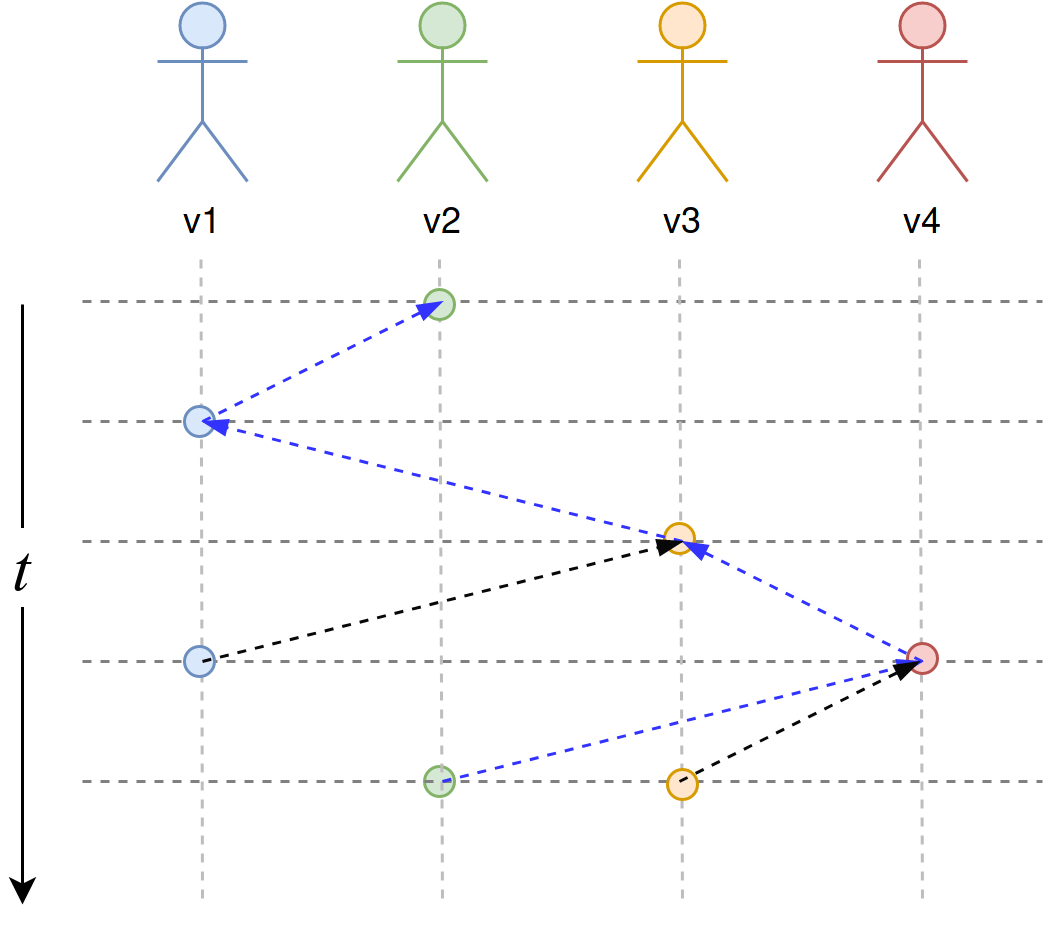
\includegraphics[width=0.8\columnwidth]{cbc-example}
  %\captionsetup{justification=centering}
    \caption{\gls{cbc} blockchain example}
	\label{fig:example}
\end{figure}

\fig{fig:example} shows a small example of a \gls{cbc} execution
over a blockchain. Four nodes are pictured. Colored circles are messages sent by
validators, dotted arrows show their justifications. The selected blockchain is
depicted with blue arrows. It is obtained by running the \gls{ghost} algorithm
on the pictured view of the network, and would be the estimate of a new message
sent by an honest validator that has this view.

\fig{fig:example2} examplifies validator \(v_1\) producing a new message
and the resulting new blockchain. An honest node includes all the latest
messages it has received (including its own last message). When a validator does
not include its own messages in its justification, it is considered as an
\textit{equivocator}, does not follow the protocol, and could be punished by
the network for such a behavior. Note that validator \(v_1\) does not equivocate
because its first message is in the justification of \(v_2\)'s first message,
and \(v_1\) has this message in the justification of its second message. It is
said that \(v_1\)'s first message is in the \textit{dependency} of its later
messages.

\textit{Finality} is a key concept to understand for this project. A block is
considered as finalized in a view if it cannot be removed from the blockchain by
receiving new messages from honest nodes. In this project, a block is considered
as finalized when a \textit{safety oracle} \cite{abstractCBC} is detected on it.
Without entering into too much detail, the safety oracle that is used marks
blocks as safe when at least \(50\%\) of the validators acknowledge that they
saw the block in their chosen blockchain. \todo{more details, more precise?}

\begin{figure}[h]
	\centering
	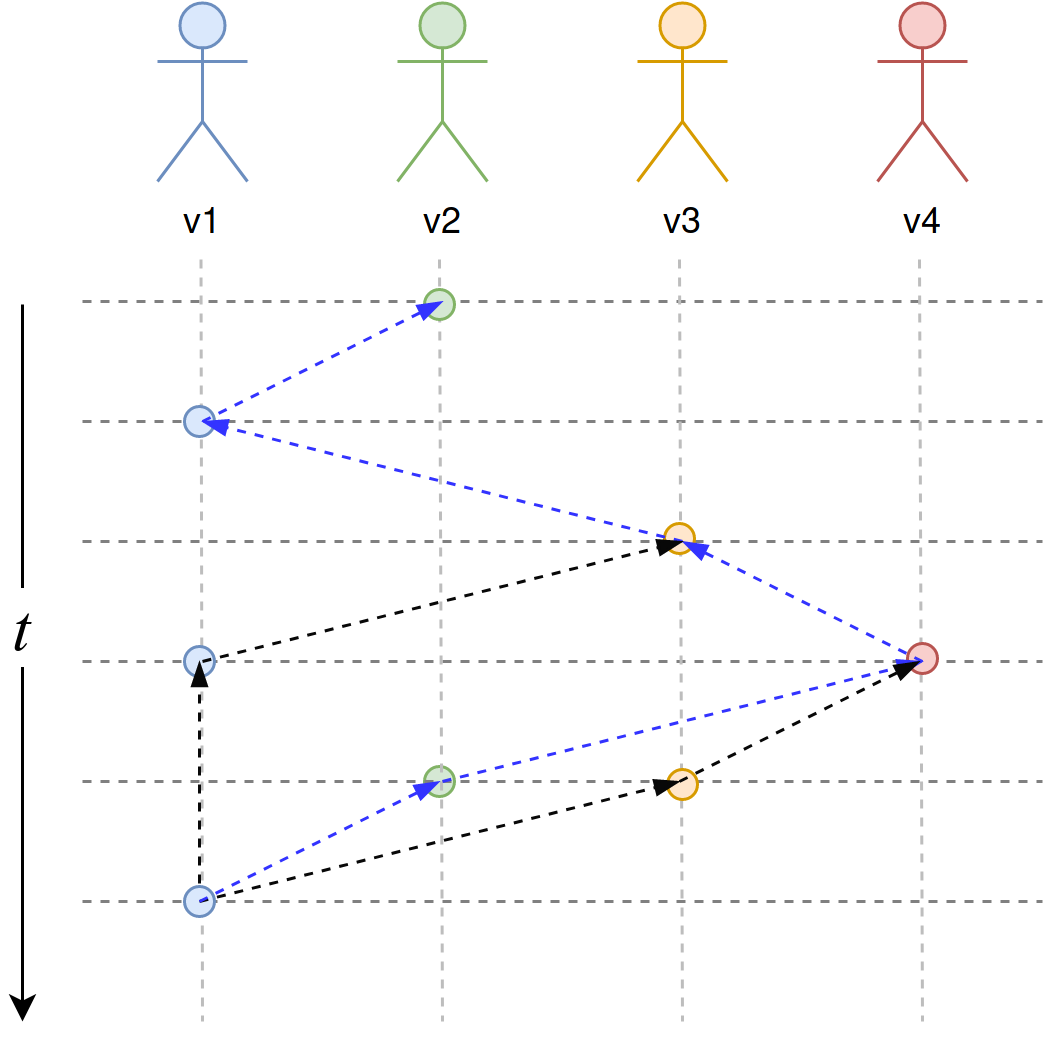
\includegraphics[width=0.8\columnwidth]{cbc-example-2}
  %\captionsetup{justification=centering}
    \caption{\gls{cbc} blockchain example 2}
	\label{fig:example2}
\end{figure}

\FloatBarrier
\subsection{Differences between \gls{cbc} Casper and \gls{pow}}
\label{ssec:powVsPos}

\subsubsection{Block production}
In a \gls{pow}\cite{yellowpaper} setting, a miner can broadcast any block to the network, but the
block will only be picked up by the other nodes if it is valid. As the miner has
to work to produce a valid block, it cannot create blocks on the fly at any
time, whereas in a \gls{cbc} Casper setting, a node can broadcast blocks at any
time. 

\subsubsection{Timing assumption}
In a \gls{pow} protocol, the work a miner has to do to create a block is
parametrized by the difficulty of the cryptographic puzzle it has to solve. This
difficulty is set in such a way that it takes a certain time -on average- to
solve the puzzle. On the contrary, the \gls{cbc} Casper protocol family does not
make any timing assumption.

\subsubsection{Spam}
The two previous points imply that spamming issues are mitigated by the need to
work to produce blocks in a \gls{pow} chain. However, as there is a negligible
computational cost to produce Casper messages, a node could easily spam the
whole network.

\subsubsection{Economic majority}
\todo{cite ref, and better explanation}
As machines that are better at solving the cryptographic puzzle in a \gls{pow}
context are more expensive to buy and to operate, \todo{nah}
Economic majority is however built in the \gls{cbc} Casper protocol, in the form
of the weight that validators have.

\subsubsection{Building strategy}
In order to receive a reward for its work, a miner wants a block it has produced
to be included in the main chain. A \gls{pow} protocol usually states that the
chain with the most total difficulty is the main one. Therefore, a miner is
incentivised to build on top of the main chain. 
In a Casper setting, as there is no such incentive, a validator could build on
any chain, or even on its own chain.


\begin{table}[H]
    \centering{
        \begin{tabular}{|l|p{47mm}|p{47mm}|}
            \hline
            & \gls{pow} & \gls{cbc} Casper \\
            \hline
            Block production & Miners can publish blocks if the can prove they
            worked for it & Nodes can publish blocks at any time \\
            \hline
            Timing assumption & Work is a proxy for timing & None \\
            \hline
            Spam & Work removes the possibility to spam & Negligible
            computationnal costs to produce blocks imply potential spam \\
            \hline
            Economic majority & Work is a proxy for economic majority & Economic
            majority \\
            \hline
            Building strategy & Nodes are incentivised to build on the longest
            chain because they have to work to build blocks & No clear
            incentive to build on the longest chain \\
            \hline
        \end{tabular}
        %\captionsetup{justification=centering}
        \caption{Summary of key differences between \gls{pow} and \gls{pos}}
        \label{fig:keyDiffPowPos}
    }
\end{table}

\section{Main problematic}
\todo{rename section}
As seen in \ssec{ssec:powVsPos}, many real-life implementation points are still
to define in order to have a practical \gls{cbc} Casper blockchain. One main
problem that arises is the selection of a block building strategy. This project
will try to propose a model to compare strategies, as well as a framework that
allows one to easily implement new strategies and discuss their performances
based on the proposed model.
Basic strategies that have predictable outputs will be implemented as well, in
order to validate the functionality of the framework.

\section{\texttt{core\_cbc}}
\texttt{core\_cbc} a Rust implementation of the \gls{cbc}-Casper, made by
TrueLevel \todo{introduce somewhere}. It implements the consensus algorithms proposed in the paper and
offers an abstract structure that can be used to create consensus on any value.

\section{Parity Ethereum}
\todo{remove redundancy in this chapter}
\todo{parity networking/gossiping layer research?}
Parity is a Rust Ethereum client. It includes a \textit{Pluggable Consensus}
module that allows one to easily add new consensus protocols by implementing an
interface.  At first, the goal of this project was to implement a small bridge
between the Parity module and the \texttt{core\_cbc} implementation to test block creation
strategies in a pseudo real-like manner. The implementation of the bridge was
not as straight forward as planned so it has been decided to cut it out and test
strategies without mimicking the network and client settings.

\subsection{Background work}
During the early stages of this project, a clear objective was set: to be able
to run a Casper \textit{testnet} with Parity custom nodes. Some work has been
done for the implementation of the \texttt{core-cbc} library into Parity, but
that was left to people that had a better understanding of the underlying
library. Furthermore, \todo{rephrase "a lot of"} a lot of effort had been
injected in the creation of a Docker infrastructure in order to easily deploy,
connect and monitor multiple custom Parity nodes on a single machine in order to
experiment with different message building strategies. The choice of using
Docker was made because there was a  possibility to work on the UniNE clusters,
which happen to work well with containerized software. After seeing that the
Parity implementation would take too much time to be completed, and therefore
might be unusable for this thesis, it has been decided to evaluate strategies
inside the \texttt{core-cbc} library instead of the more real-life-like setting
that is a Parity testnet. The core library was still being implemented at the
time and further testing was needed. The main disadvantage of doing the experimentations in
the library is that the whole network latencies and topology are not taken into
account. However, a non-negligible advantage of implementing strategies in the
core library is that it will be easier to test them on consensus values that are
not only blockchains.

\subsection{Local testnet}
Scripts that create and manage two local nodes have been written. They launch 2
Parity instances with the \gls{cbc}-Casper consensus engine, and connect them
to each other. Each node has a user account to send transactions, as well as a
sender account, that can act as a validator in a Casper sense. Currently, each
node produces a block every 10 seconds. This is a basic strategy that enabled
further testing of the Parity inclusion of the \texttt{core-cbc}.

\subsection{Docker testnet}
Testing at a larger scale than two local instances was needed. The possibility
to access a cluster at the UniNE was discussed and the more straightforward way
to run programs on the cluster is to have containers. It was therefore decided
to create a more complex infrastructure using Docker containers.
\texttt{docker-compose} scripts were created to achieve this goal. An arbitrary
number of containers can be created at once and inter-connected in two different
ways:
\begin{itemize}
    \item fully connected;
    \item ring.
\end{itemize}

\begin{figure}
	\centering
	
\includegraphics[width=0.8\columnwidth]{rings}
  %\captionsetup{justification=centering}
    \caption{Parity nodes topologiess implemented in the Docker testnet. Ring
    layout (left), fully connected (right)}
	\label{fig:example2}
\end{figure}

The created nodes have the same types of accounts as for the local testnet.
In the fully connected setting, each node is connected to every other node. In
the ring case, each node is connected to two other nodes in a circular manner.
Those were the two first layouts that were implemented for simplicity. It was
thought to add new layouts afterwards in order to match more precisely the real
network topology of the Ethereum \textit{mainnet}. However, because the Parity
implementation was deemed too time consuming to be used before the end of this
project, no further efforts have been put in that direction. Nevertheless, the
software architecture is in such a state than adding and removing topologies is
easily done through abstract structures.

\chapter{Strategies Evaluation}
\label{chap:strategies}

\section{Modelisation}
\subsection{Metrics}
A way to rationaly compare strategies is needed in order to discuss their
relative strengths and weaknesses. Three main characteristics will be used for
that:
\begin{itemize}
        \item latency;
        \item number of nodes;
        \item overhead.
\end{itemize}

\subsubsection{Latency}
The latency is the number of messages needed to finalize a block. Ideally, you
want to have a latency as low as possible to reach finality as soon as possible.
The latency is a way to measure liveness in a blockchain system. If it is low,
then the system is considered more "live", as fewer messages are needed in order
to confirm a transaction, and therefore less time.

\subsubsection{Number of nodes}
The number of nodes is quite straightforward; it is the number of nodes that are
in the validator set. This number should be as high as possible to guarantee
decentralization and therefore safety.

\subsubsection{Overhead}
The overhead is the number of messages that are sent over the network between
one step of the consensus and the next. It should be as low as possible to keep
the costs in bandwidth low.

\subsubsection{Example}

\begin{figure}[H]
	\centering
	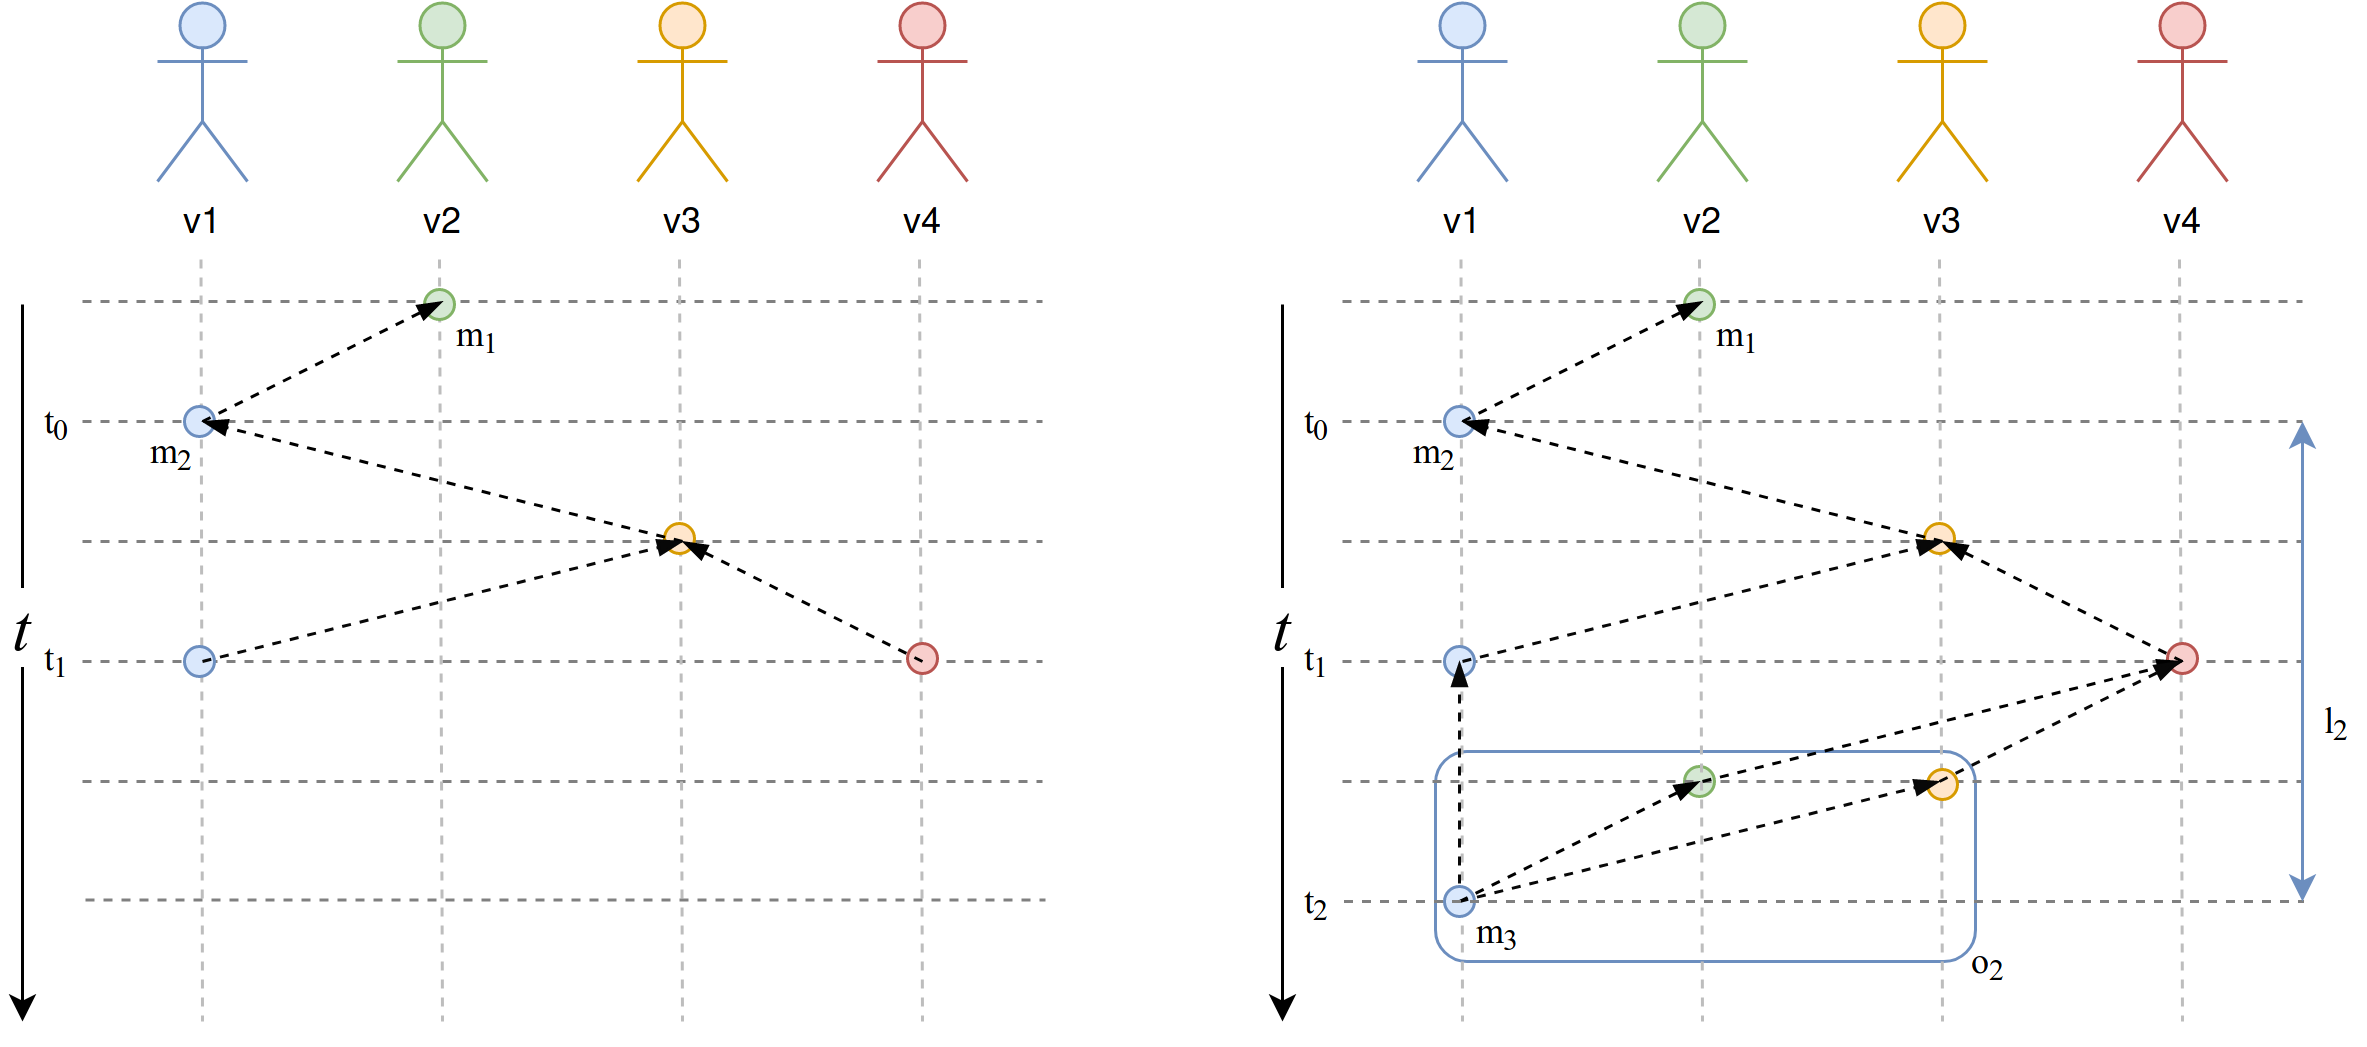
\includegraphics[width=\columnwidth]{metrics-example}
  \captionsetup{justification=centering}
    \caption{Metrics computation example}
	\label{fig:metricsSchema}
\end{figure}

Figure~\ref{fig:metricsSchema} describes how the computation of the metrics
takes place. The left half of the figure shows an initial view of the system. At
time \(t_1\), message \(m_1\) is finalized. The right half of the figure shows a
view of the system at \(t_2\), time at which \(m_2\) is finalized. The latency
of \(m_2\) is \(l_2\), the difference of heights between \(m_3\) and \(m_2\). In
this example, \(l_2 = 4\). \(o_2\), the overhead for \(m_2\), is the number of
messages that have been sent between \(t_1\) and \(t_2\), \(t_1\) being the time
at which the previous message has been finalized and \(t_2\) the time at which
the current message is finalized. In the example, \(o_2 = 3\).

\subsection{Tradeoff triangle/Trilemma}
In a standard consensus protocol, the three metrics form a trade-off triangle in
kind of a "pick two" fashion. \todo{not a pick two} \gls{cbc}-Casper has no
assumptions on timings, sources, contents, destinations of the messages that are
exchanged, and can therefore explore the whole trade-off space. This project
aims to find strategies that span the entierty of the triangle and 
\todo{finish sentence what}

\subsection{Basic model}
\label{ssec:model}
The first model that has been chosen for the evaluation is the following:

\[1 = s_n \cdot \frac{1}{n} + s_l\cdot l + s_o\cdot o\]

This model binds 3 scores \(s_x\) to their respective variables \(x\).
Variables are as follows:
\begin{itemize}
    \item \(n\) the number of nodees;
    \item \(l\) the latency;
    \item \(o\) the overhead.
\end{itemize}
The higher the score \(s_x\) is, the more its related variable is dominant
in the strategy and therefore the closer to a corner of the triangle the strategy is.
\(\frac{1}{n}\) is used because a large number of nodes is wanted.
This model is a basic one, where everything is linear. It is probably not accurate but
will serve as a base for a closer to reality one once data have been plotted using
this model.
\todo{why 1/n, why everything linear?}

\subsection{Model Evaluation}
After running the strategies in the simulation environment, metrics for \(n\),
\(l\) and \(o\) will be recorded. Then, for multiple runs, a linear regression
will be performed in order to find the scores \(s_x\).

\section{Strategies}
\label{sec:strategies}

The following strategies were proposed in order to visit the entierty of the
trade-off triangle:
\begin{itemize}
        \item round-robin;
        \item randomness;
        \item double round-robin;
        \item triple round-robin;
        \item overhead.
\end{itemize}
These strategies should allow one to visit the whole triangle and to discuss
their respective strength and weaknesses. The following sections describe the
strategies as well as their expected locations in the triangle.

\subsection{Round-robin}
The first strategy that comes to mind is a simple round-robin. Nodes send
messages one after the other, in a fixed order.
\todo{talk about real life implications? aka synchronize all nodes?,\ldots and
that for every strategy}

\subsection{Randomness}
The next strategy is the simplest to think of: complete randomness. Using fixed
probability density functions, nodes chose when to create messages and to which
other validator to send them.

\subsection{Double Round-robin}
In this setting, two nodes send messages at the same time, in a fixed order. If
the two nodes that send messages at the same step are at opposite places in the
set of validators \todo{explain better}, the latency to finality is supposedly
half as much as the simple round-robin strategy. The overhead is however
doubled.\todo{add that we could have a triple rr, quadrr, \ldots}

\subsection{Triple Round-robin}
This strategy is similar to the Double round-robin, except that three nodes send
a message a each step. It was decided to add this strategy at a later stage of
the project in order to have intermediate comparison points between the Double
round-robin and the Maximal overhead strategy. As for the Double round-robin
strategy, the latency should be divided by three compared to the simple
round-robin and the overhead should be three times higher.

\subsection{Maximal Overhead}
This strategy is the most expensive in terms of bandwidth; at each step, each
validator sends a message to the others. This example strategy should give a
baseline value for the maximum overhead that is reachable in the tradeoff
triangle.

\subsection{Bottom-up strategies}
All the previous strategies (except the Arbitrary one) can be viewed as
"top-down" strategies, as there has to be a way for nodes to be synchronized.
Strategies that are easier to implement from a real-life point of view would be
strategies that only depend on the data available on a node. For exemple, a node
could keep track of the whole state of the finalization of messages, and only
publish a message itself when it facilitates the finalization. That kind of
strategy has not been implemented but the testing and scoring framework allows
one to easily add them.

Such strategies should implement incentives for the nodes not to spam the
network and include mechanisms to slash nodes not following some rules the
strategies dictate.

\section{Experimentations}
Over the duration of this thesis, the \texttt{core-cbc} library has included a
test framework called \texttt{proptest}. The testing framework that has been
implemented includes ways to simulate the behavior of the Casper protocol over
multiple nodes and thousands \todo{numbers} of blocks. At the time of the
writing, the simulations do not include networking latencies.

\subsection{\texttt{proptest}}
The \texttt{proptest} implementation is able to run blockchain simulations off
the following parameters:
\begin{itemize}
    \item Number of validators;
    \item Terminating condition;
    \item Sender strategy;
    \item Receiver strategy.
\end{itemize}

\subsubsection{Number of validators}
This parameter is quite straightforward, it is the number of nodes that can
validate blocks.

\subsubsection{Terminating condition}
The terminating condition is a predicate that tells whether or not the simulation has
reached an end. In our case, the end of the simulation is reached when at least
one node finds a safety oracle for a blockchain that has an height of 4.
\todo{why 4}

\subsubsection{Sender strategy}
The sender strategy selects one or more nodes that will create new messages and
forward them to the rest of the network. All the basic strategies that have been
presented in Section~\ref{sec:strategies} are implemented as Sender strategies.
New strategies (including bottom-up ones) can be easily implemented as well.

\subsubsection{Receiver strategy}
Receiver strategies select a set of validators that receive messages created by
Sender strategies. Two strategies have been implemented for now: 
\begin{itemize}
        \item All receivers;
        \item Some receivers.
\end{itemize}

The \textit{all receivers} strategy broadcasts messages to each other validator.
The \textit{some receivers} strategy sends a message to \(1\) or more validator,
using an uniform probability density function.  As of now, none of the
implemented strategies are a good modelisation of a typical Ethereum network and
this will be fixed at a later iteration.  Nonetheless, these strategies offer
two extreme points on the spectrum of the network topology: a fully connected
one without latency (\textit{all receivers}), and a random one (\textit{some
receivers}) and will be both taken into account to compare the sender
strategies.

\subsection{Metrics measurements}
Metrics are not computed as-is in the \texttt{proptest} implementation. Simpler
datas are logged into \texttt{csv} files, and are processed by a \texttt{Python}
script. \todo{what data} This two steps processing permitted the generation of
data before having a precise definition of the metrics. It also permits to vary
the way metrics are recorded. For example, from the same log file, you could
extract metrics only when the last step of the consensus is reached, or have an
average of the metrics at each step of the consensus.

\subsection{Tests}
Table~\ref{fig:recapTests} summarizes which tests have been run.
All of them have the same terminating condition, which is reached when at least a
node finds a safety oracle at height 4. The number of nodes is chosen at random
in the interval \([1, 20[\). It has been decided to perform tests on this
interval because it is large enough to give an insight on the behavior of the
relations between the metrics, and small enough to reach the terminating condition in
a reasonable time (1 run with a number of nodes chosen at random takes on average 1 hour
with the Maximal overhead strategy).

\todo{renove table}

\begin{table}[H]
    \centering{
        \begin{tabular}{|c|c|c|}
            \hline
            & All receivers & Some receivers \\
            \hline
            Round-robin & \checkmark & \checkmark\\
            \hline
            Double round-robin & \checkmark & \checkmark\\
            \hline
            Maximal overhead & (\checkmark) & (\checkmark) \\
            \hline
            Arbitrary & \checkmark & \checkmark\\
            \hline
        \end{tabular}
        \captionsetup{justification=centering}
        \caption{Summary of tests that have been run. A tick in parenthesis
        implies that tests were run but that there are not many data points or
        big disparities in the distribution of the number of nodes}
        \label{fig:recapTests}
    }
\end{table}

\todo{schema with what to measure}
\todo{how the measurements take place in the code}

\section{Visualization I: All receivers}
This chapter presents a visualization of the datas obtained through the multiple
test runs with the All receivers strategy.  Each subsection shows the results
using 3 histograms, representing the raw data, followed by 3 scatter plots
picturing each metric against each other. These graphs also show a simple linear
regression as an attempt to find a relation between each metric. At the end of
the discussion of each strategy a linear regression is performed in order to
find the scores of each variable according to the model presented in
Subsection~\ref{ssec:model}.


\todo{3D plotting?}
\todo{undersampling issue?}

\subsection{Round-robin}

The distributions of the number of nodes and the latency
(Figure~\ref{fig:distRR} left and center) have the same
shapes except for the gaps every 3 steps. The resemblance in shape is explained
by the fact that the latency is strictly correlated to the number of nodes, as
expected.
The gaps will be explained in the next section, using the graphs that show
relations between variables. \todo{explain gaps}

\todo{fix center/left/right in captions and text}
\triplefigure
    {hist_nb_nodes_rr_20_nodes_4_depth_all_receivers_gen_averages}
    {hist_latency_rr_20_nodes_4_depth_all_receivers_gen_averages}
    {hist_overhead_rr_20_nodes_4_depth_all_receivers_gen_averages}
    {Distributions of the dataset. Number of nodes (left), latency (center)
    and overhead (right) \todo{change xticks label frequency}}
    {fig:distRR}

The histogram for the overhead is easy to analyse as well; the overhead is
expected to be 1 because once consensus is obtained for the genesis block, only
one message from the next validator is needed to finalize the next block.

\triplefigure
    {relation_nb_nodes_latency_rr_20_nodes_4_depth_all_receivers_gen_averages}
    {relation_nb_nodes_overhead_rr_20_nodes_4_depth_all_receivers_gen_averages}
    {relation_overhead_latency_rr_20_nodes_4_depth_all_receivers_gen_averages}
    {Relations between all the variables. Latency/Number of nodes (left),
    Overhead/Number of nodes (center) and Latency/Overhead (right)}
    {fig:relRR}

The right and center graphs on Figure~\ref{fig:relRR} do not give more insight on the
data, as the Overhead is always \(1\). On the other hand, the graph on the left
shows a clear linear relationship between the latency and the number of nodes.
The fitted line has the following equation:
\[l = 1.403402\cdot n\]
The latency is expected to be around \(1.5\cdot n\) because the finality is
reached when at least 50\% of the network has acknowledged that the whole
network has the finalized message in its justification. As pictured in the
top-left graph of Figure~\ref{fig:relRR}, the fitted line has a slightly small
slope compared to the data points due to the fact that the line is fitted to be
linear and the data points are close the origin. \todo{insert line with 1.5*n ?}

\subsection{Double round-robin}
\triplefigure
    {hist_nb_nodes_double_rr_20_nodes_4_depth_all_receivers_gen_averages}
    {hist_latency_double_rr_20_nodes_4_depth_all_receivers_gen_averages}
    {hist_overhead_double_rr_20_nodes_4_depth_all_receivers_gen_averages}
    {Distribution of the dataset. Number of nodes (left), latency (center)
    and overhead (right)}
    {fig:distDRR}
As for the simple round-robin case, the latency and number of nodes
distributions show a similar shape. The latency is less spread than for the
singl round-robin, which explains some dissimilarities between the
distributions. The distribution of the overhead presents a peak at 2, which is
expected but also shows that there are some messages that have double this
overhead, at 4. This will be explained using the following graphs. \todo{explain
outliers}

\triplefigure
    {relation_nb_nodes_latency_double_rr_20_nodes_4_depth_all_receivers_gen_averages}
    {relation_nb_nodes_overhead_double_rr_20_nodes_4_depth_all_receivers_gen_averages}
    {relation_overhead_latency_double_rr_20_nodes_4_depth_all_receivers_gen_averages}
    {Relations between all the variables. Latency/Number of nodes (left),
    Overhead/Number of nodes (center) and Latency/Overhead (right)}
    {fig:relDRR}

As for the simple round-robin strategy, the plots including the Overhead are not
of much use here, except they show that its value is 2, as it is expected. 
On the other hand, the plot on the top-left of Figure~\ref{fig:relDRR} shows a
linear relation between the number of nodes and the latency: 
\[l = 0.721750 \cdot n\]
This value is about half of the slope obtained for the same relation with the
round-robin strategy. The double round-robin strategy was supposed to show half
the latency with respect to the simple round-robin and this value is therefore
correct. The value of 2 for the overhead is also twice the overhead for the
single round-robin and confirms the hypothesis.
    

\subsection{Triple round-robin}
The triple round-robin strategy shows  the same kind of information as the
double round-robin one. The overhead is 3 for almost all cases (this will be
discussed later), and the number of nodes and latency are lineraly correlated.
\triplefigure
    {hist_nb_nodes_triple_rr_20_nodes_4_depth_all_receivers_gen_averages}
    {hist_latency_triple_rr_20_nodes_4_depth_all_receivers_gen_averages}
    {hist_overhead_triple_rr_20_nodes_4_depth_all_receivers_gen_averages}
    {Distributions of the dataset. Number of nodes (left), latency (center)
    and overhead (right)}
    {fig:distTRR}

The relationship with the overhead are again not of much use because its value
is always 3. Again, there is a linear relationship between the latency and the
number of nodes, which follows this equation:
    \[l = 0.496152 * n\]
The slope is a third as the slope for the simple round-robin strategy. Moreover
the overhead is three times larger for the triple round-robin than it is for the
simple.
\triplefigure
    {relation_nb_nodes_latency_triple_rr_20_nodes_4_depth_all_receivers_gen_averages}
    {relation_nb_nodes_overhead_triple_rr_20_nodes_4_depth_all_receivers_gen_averages}
    {relation_overhead_latency_triple_rr_20_nodes_4_depth_all_receivers_gen_averages}
    {Relations between all the variables. Latency/Number of nodes (left),
    Overhead/Number of nodes (center) and Latency/Overhead (right)}
    {fig:relTRR}

\subsection{Maximal overhead}
This strategie aims to reduce latency to its minimum, which is shown in the
top-right plot on Figure~\ref{fig:distOverhead}. The distributions of the number
of nodes and overhead are of the same shape because they are lineraly
correlated, as will be shown in the next paragraph. 
Note that the experiments have been run with a lower number of nodes because the
simulations for a large number of nodes takes a large amount of time. The
simulations are currently implemented following the mathematical formulae found
in \todo{VLADS PAPER} and not yet optimized. For completeness's sake, a few runs
have been performed with the same amount of nodes as for the other experiments
to show whether or not there were divergences. It turned out that there was not
such divergences. 
\todo{talk about why the number of nodes is not even}
\triplefigure
    {hist_nb_nodes_overhead_10-20_nodes_4_depth_all_receivers_gen_averages}
    {hist_latency_overhead_10-20_nodes_4_depth_all_receivers_gen_averages}
    {hist_overhead_overhead_10-20_nodes_4_depth_all_receivers_gen_averages}
    {Distribution of the dataset. Number of nodes (left), latency (center)
    and overhead (right)}
    {fig:distOverhead}

The top-right plot on Figure~\ref{fig:relOverhead} clearly shows a linear
dependency between the number of nodes and the overhead. The relation is \(o =
n\), as it is expected.
The two other plots on the same Figure only confirm that the latency equals 2,
which is the minimum that can be reached, as there needs to be two steps to
finalize a message. During the first step, all nodes acknowledge they have seen
a message, and the second step confirms that everyone has seen the other nodes
acknowledgments.

\triplefigure
    {relation_nb_nodes_latency_overhead_10-20_nodes_4_depth_all_receivers_gen_averages}
    {relation_nb_nodes_overhead_overhead_10-20_nodes_4_depth_all_receivers_gen_averages}
    {relation_overhead_latency_overhead_10-20_nodes_4_depth_all_receivers_gen_averages}
    {Relations between all the variables. Latency/Number of nodes (left),
    Overhead/Number of nodes (center) and Latency/Overhead (right)}
    {fig:relOverhead}

\subsection{Arbitrary}
This strategy is the only one that uses a random factor and that can be
considered as a "bottom-up" strategy.

\triplefigure
    {hist_nb_nodes_arbitrary_20_nodes_4_depth_all_receivers_gen_averages}
    {hist_latency_arbitrary_20_nodes_4_depth_all_receivers_gen_averages}
    {hist_overhead_arbitrary_20_nodes_4_depth_all_receivers_gen_averages}
    {Distribution of the dataset. Number of nodes (left), latency (center)
    and overhead (right)}
    {fig:distArbitrary}
\triplefigure
    {relation_nb_nodes_latency_arbitrary_20_nodes_4_depth_all_receivers_gen_averages}
    {relation_nb_nodes_overhead_arbitrary_20_nodes_4_depth_all_receivers_gen_averages}
    {relation_overhead_latency_arbitrary_20_nodes_4_depth_all_receivers_gen_averages}
    {Relations between all the variables. Latency/Number of nodes (left),
    Overhead/Number of nodes (center) and Latency/Overhead (right)}
    {fig:relArbitrary}


\subsection{Fitting of the basic model}
Fitting the basic model described in \todo{section} to the data gives the
following result.

\begin{table}[H]
    \centering{
        \begin{tabular}{|c|c|c|c|}
            \hline
            Sending Strategy & \(s_n\) & \(s_l\) & \(s_o\) \\
            \hline
            Round-robin & 0.0 & 0.0 & 1.0\\
            \hline
            Double round-robin & 1.435 & 0.055 & 0.162\\
            \hline
            Triple round-robin & 1.686 & 0.084 & 0.091\\
            \hline
            Maximal overhead & 0.0 & 0.5 & 0.0\\
            \hline
            Arbitrary & 2.556 & 0.026 & 0.002\\
            \hline
        \end{tabular}
        \captionsetup{justification=centering}
        \caption{Raw fitted values for the simple model, rounded to the 3rd
        decimal place}
        \label{fig:recapTests}
    }
\end{table}

The scores obtained for the round-robin and the maximal overhead strategies are
the expected ones. The round-robin strategy optimizes the overhead (one message
per new finalized block) and the latency evolves linearly with the number of
nodes and is therefore bad. The score for the number of nodes will be discussed
later in this chapter. The maximal overhead strategy shows that it maximizes the
latency (which is \(2\), the minimal value for the latency) and therefore the
rest of the scores are non influential.
For the double and triple round-robin strategies, the variation for the overhead
and the latency scores, compared to the ones for the round-robin are also in
accordance with what is expected; the latency decreases when the number of round
augments and the overhead increases along with the number of nodes sending
messages in a single round.
\subsubsection{Number of nodes}
The main problem with these results is the evolution of the score for the number
of nodes, particularly for the arbitrary strategy. Based on the observations
made in \todo{section}, the arbitrary strategy clearly is worse than the other ones for
the latency and overhead. That is reflected with the values obtained for their
respective scores. The main issue with it is that the score for the number of
nodes is used as a buffer for how well the two other variables perform in a set
strategy. Indeed, the model forces the relation between the scores and the
variables, and if the scores for both the latency and the overhead are low, the
score for the number of nodes is forced to be high.

\begin{figure}[H]
    \centering
    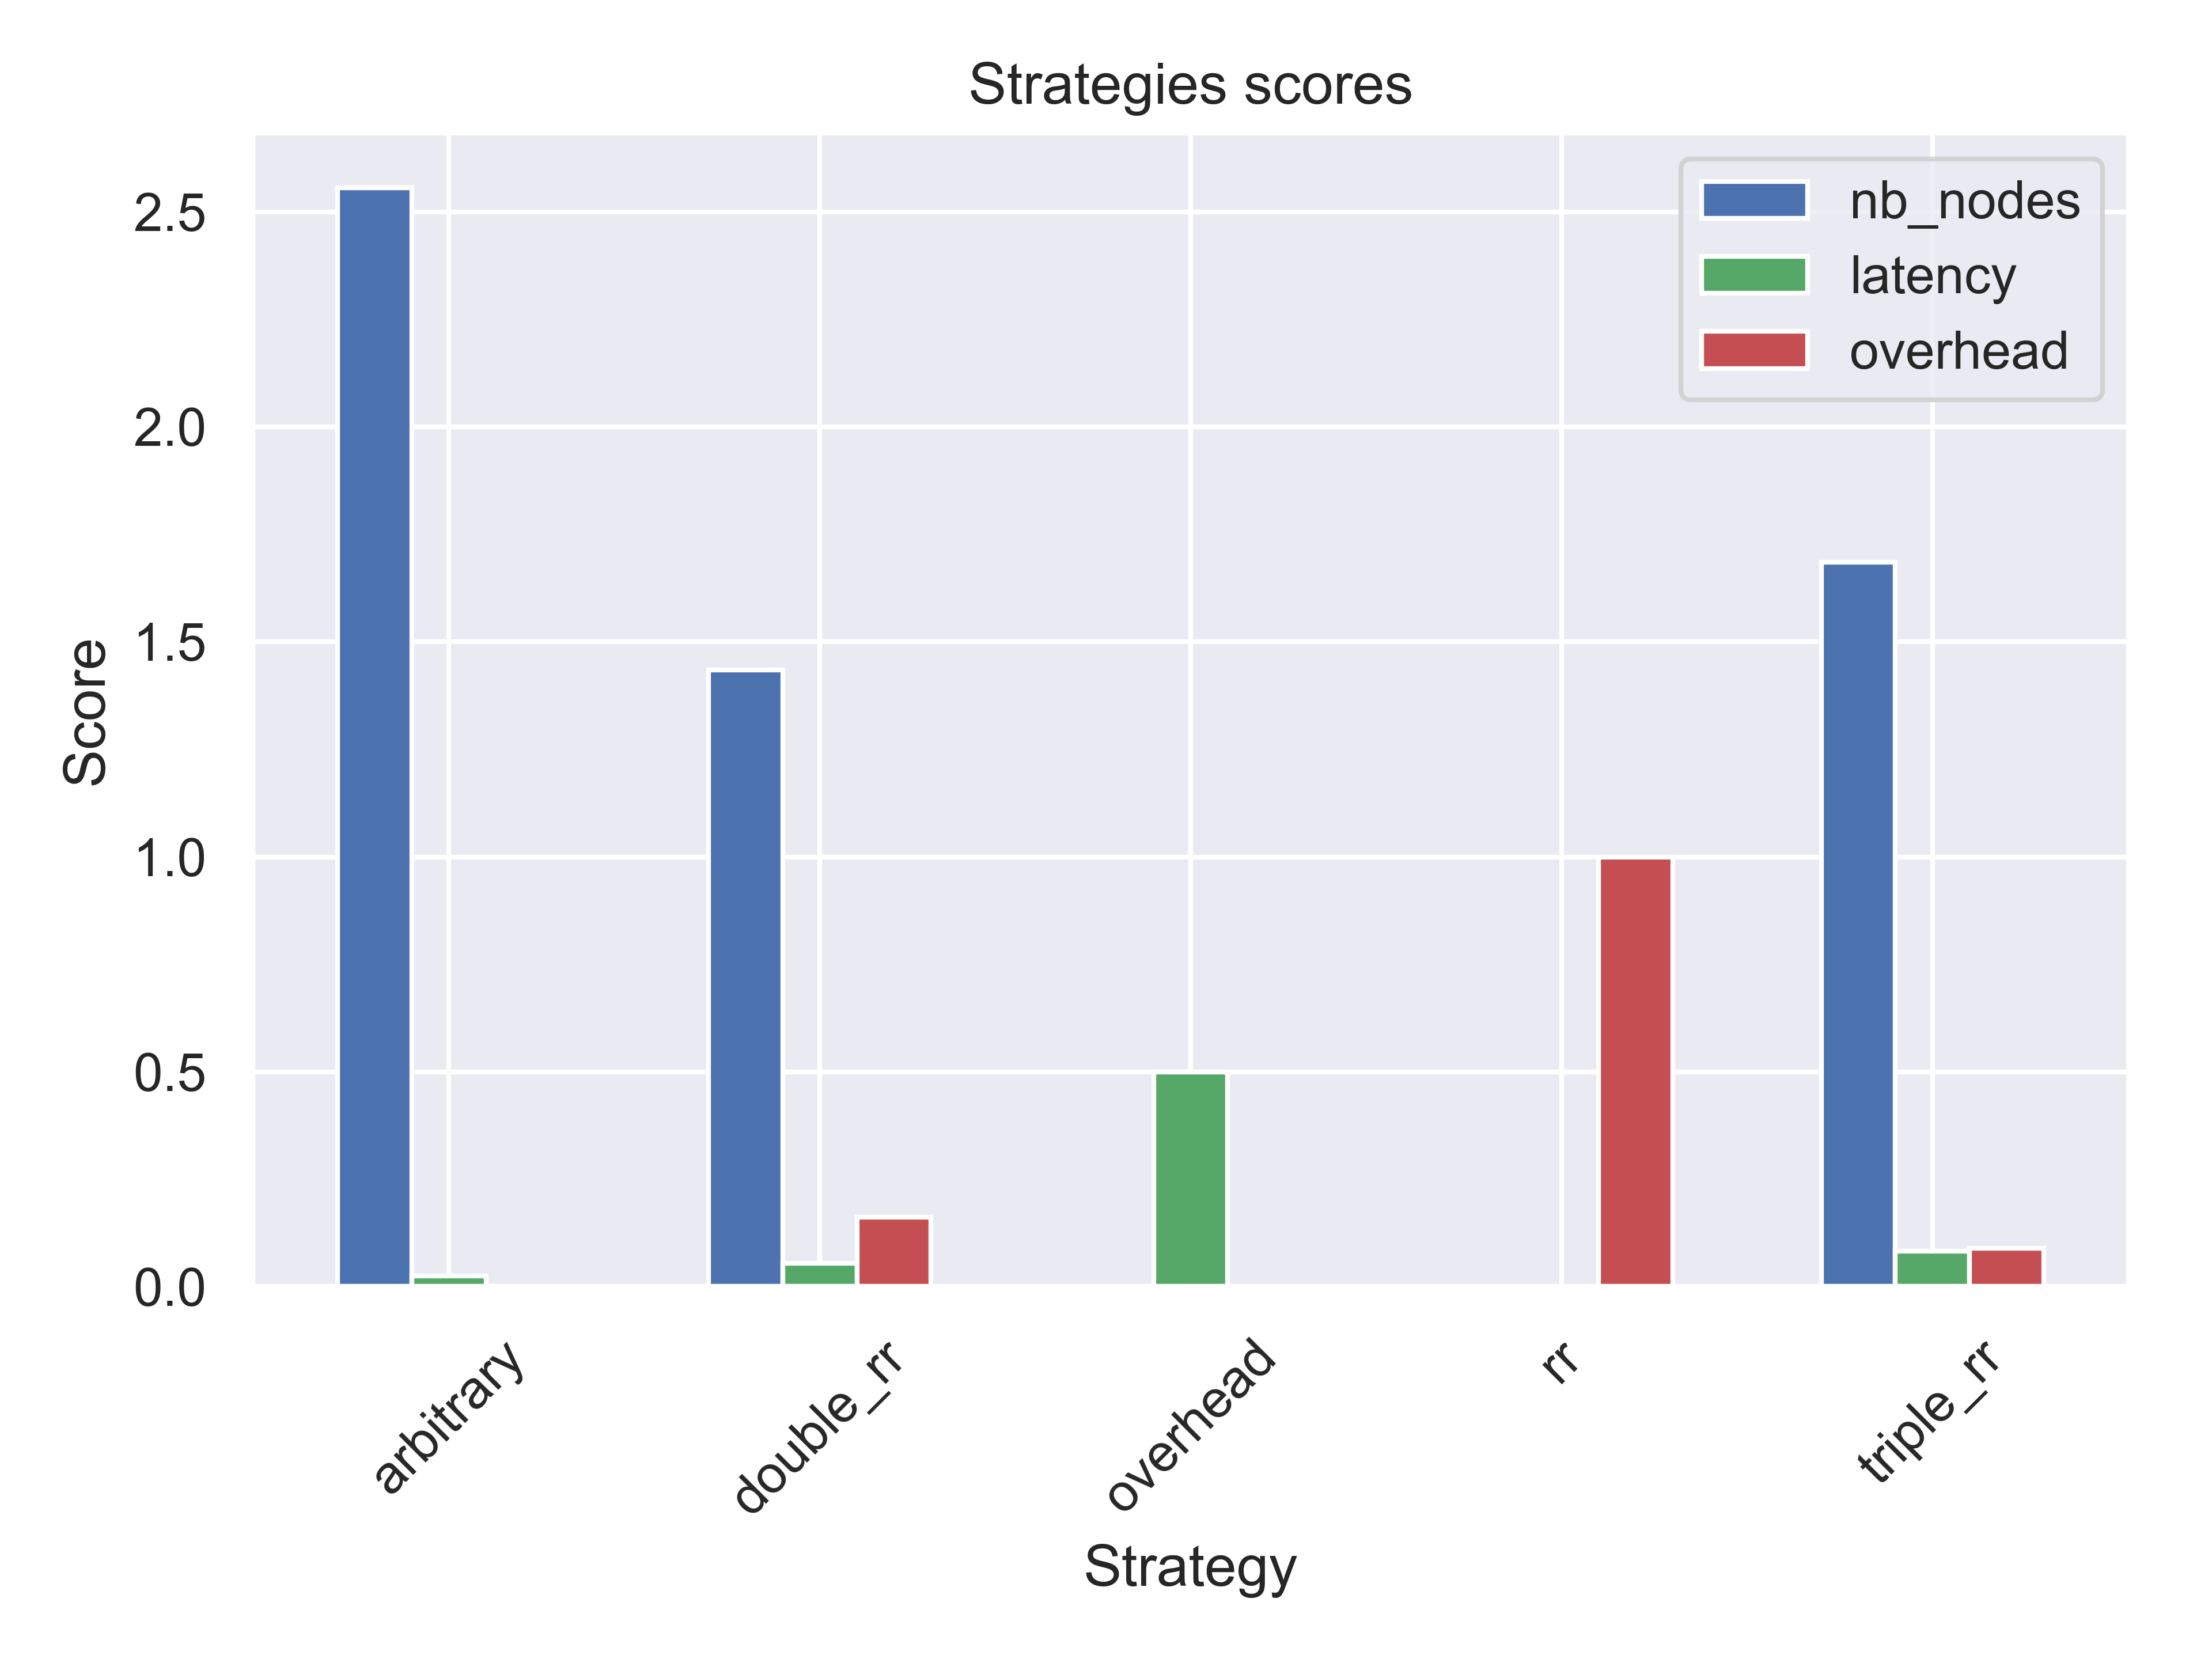
\includegraphics[width=0.8\columnwidth]{final_plot_basic_model}
    \captionsetup{justification=centering}
    \caption{Raw fitted calues for the simple model. The strategies are listed
    on the x-axis and their scores are plotted along the y-axis. \todo{prettify
    the x-axis and bar legend}}
    \label{fig:recapTestsPlot}
\end{figure}

%\begin{table}[H]
%    \centering{
%        \begin{tabular}{|c|c|c|c|}
%            \hline
%            Sending Strategy & \(s_n\) & \(s_l\) & \(s_o\) \\
%            \hline
%            Round-robin & 0.0 & 0.0 &
%            1.0\\
%            \hline
%            Double round-robin & 0.119 & 0.036 & 0.601\\
%            \hline
%            Triple round-robin & 0.404 & 0.082 & 0.401\\
%            \hline
%            Maximal overhead & 0.0 & 0.987 & 0.0\\
%            \hline
%            Arbitrary & 0.861 & 0.035 & 0.106\\
%            \hline
%        \end{tabular}
%        \captionsetup{justification=centering}
%        \caption{Raw fitted values for the simple model, rounded to the 3rd decimal}
%        \label{fig:recapTests}
%    }
%\end{table}
%
\begin{figure}[H] 
    \centering
    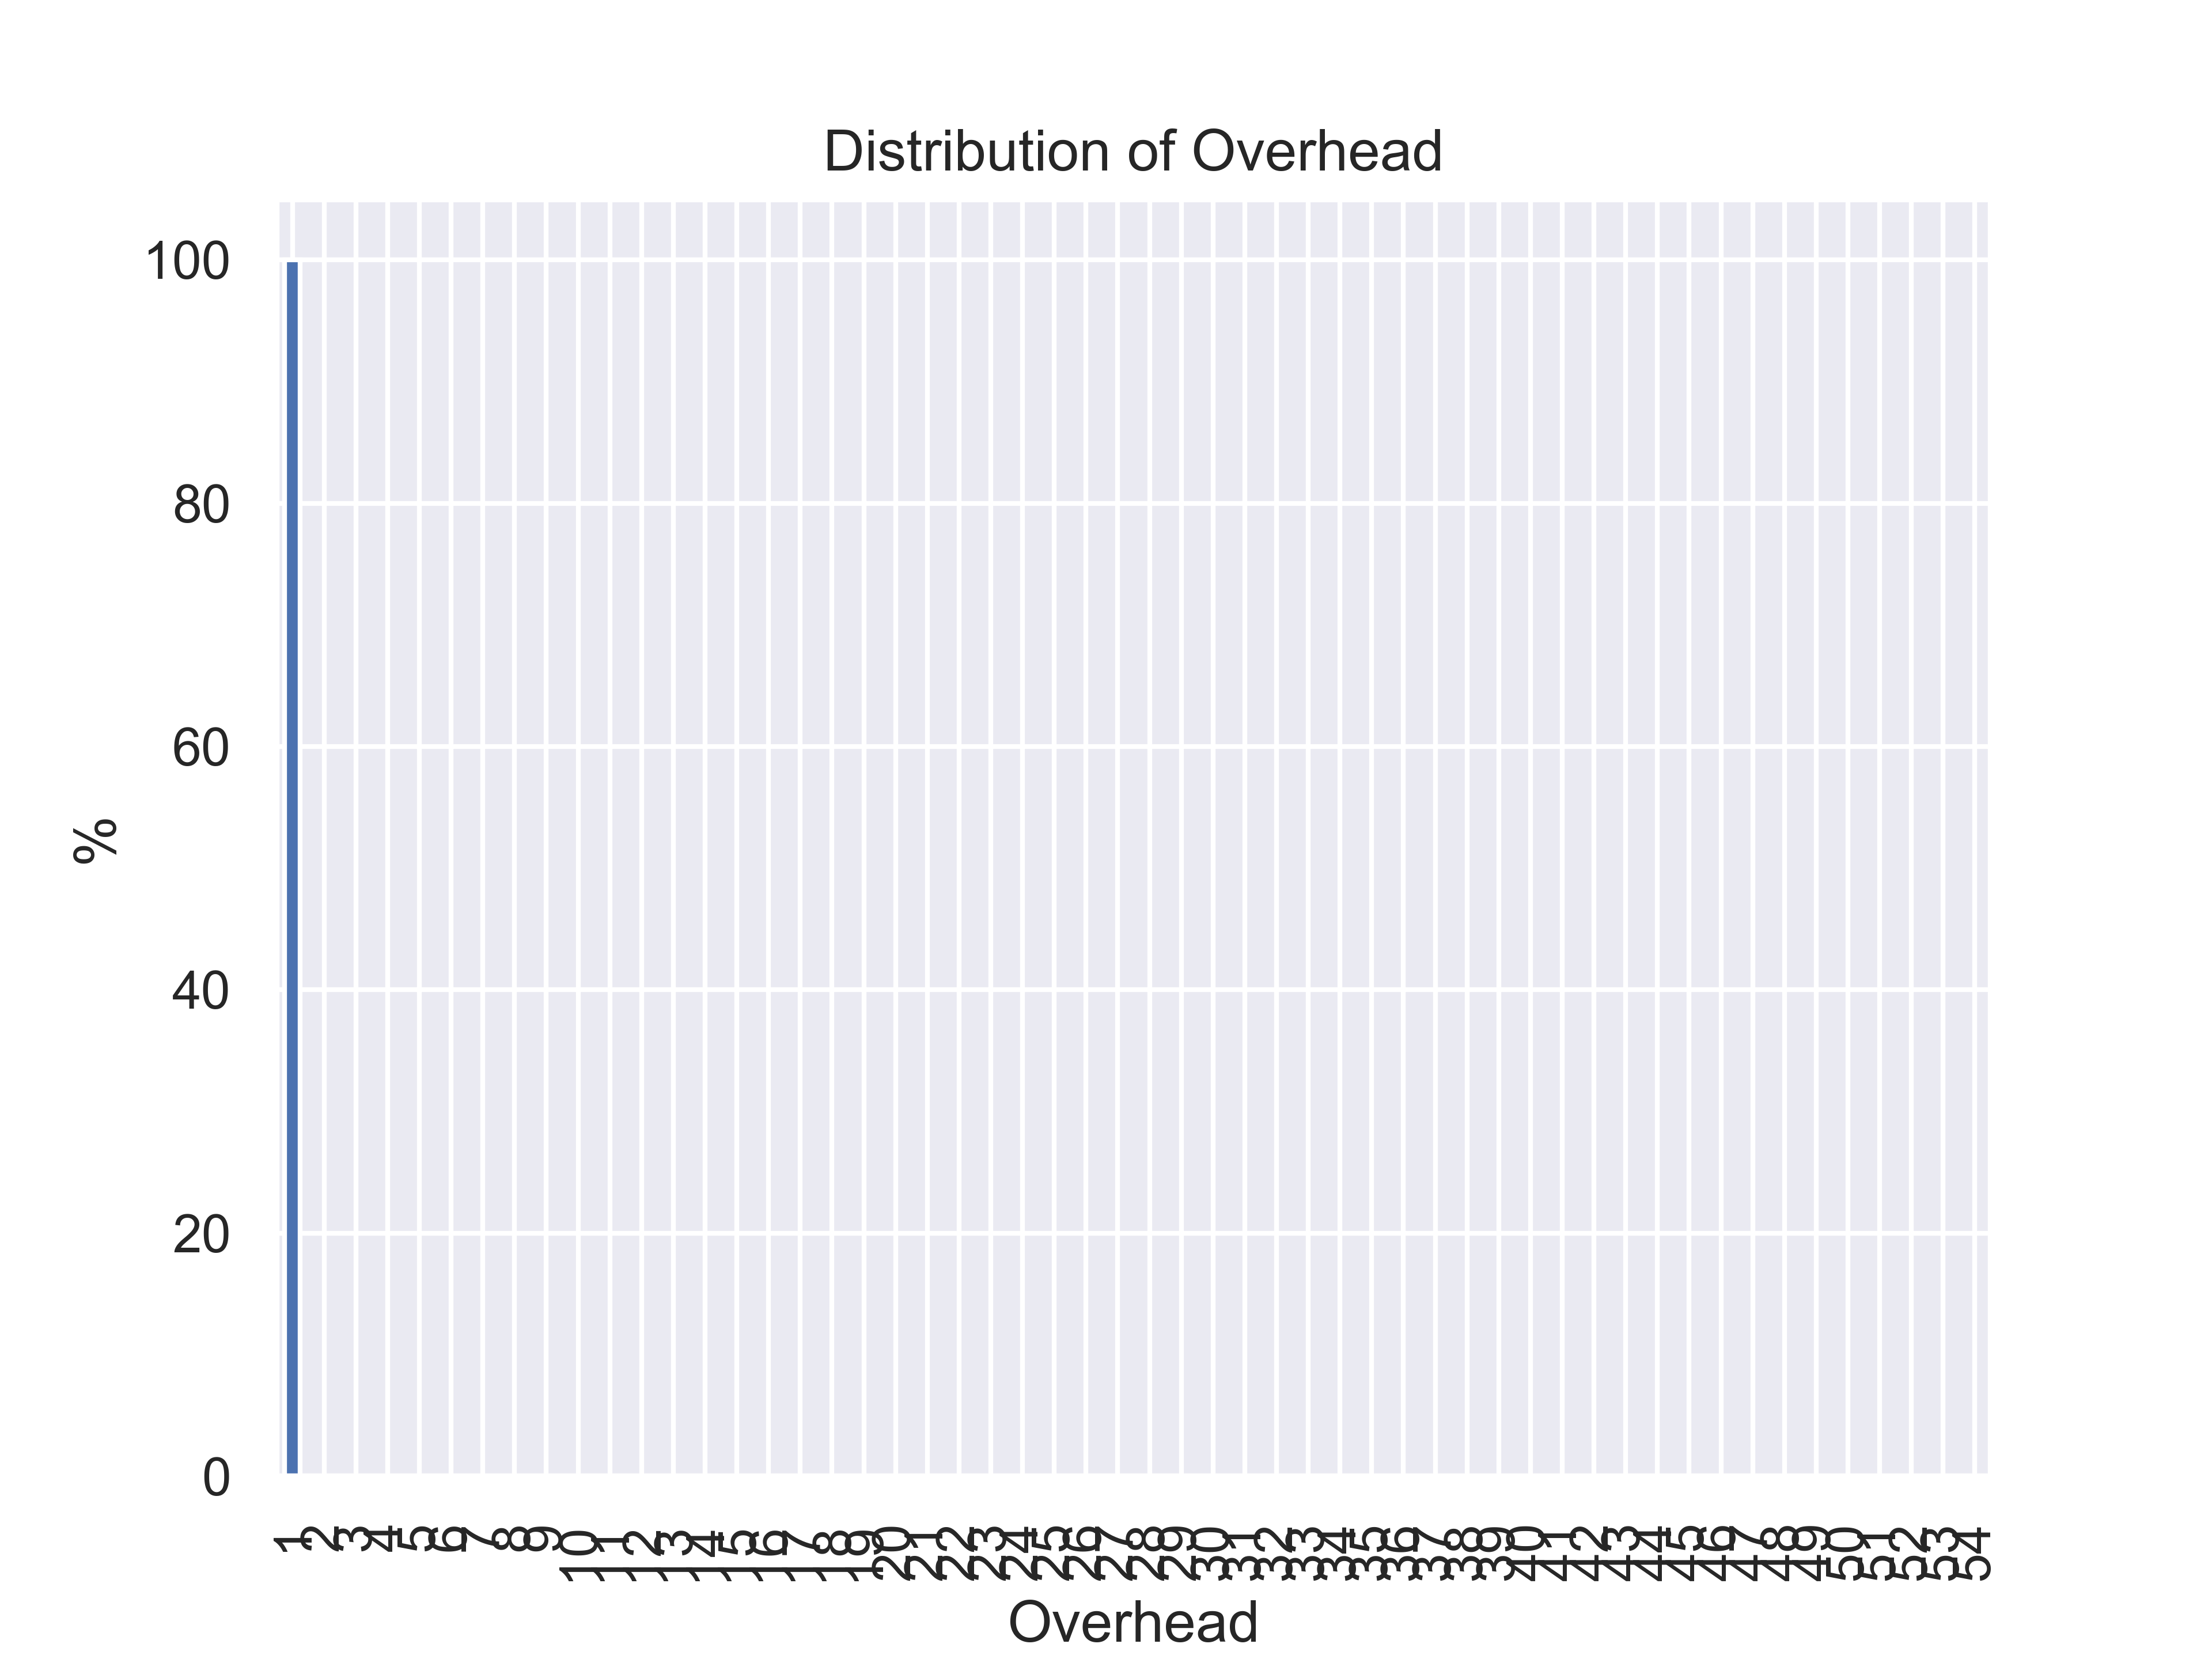
\includegraphics[width=0.8\columnwidth]{hist_overhead_rr_20_nodes_4_depth_all_receivers_gen_averages}
    \captionsetup{justification=centering}
    \caption{Histogram of the overhead. Round-robin and all receivers strategies}
    \label{fig:relOverheadLatencyRR}
\end{figure}



\subsection{Improvements of the basic model and new fitting}

\section{Analysis}
\todo{why the model is bad according to the number of nodes}

\todo{here will be a table containing all the fitted lines values and a
comparison and explanation of the behaviors that are observed}

\section{Future works}

\chapter{Conclusion}
\label{chap:conclusion}

This project aimed at finding a way to compare block building strategies for a
\gls{cbc} Casper blockchain protocol. Based on a core library implementing the
abstract structure for a \gls{cbc} Casper blockchain, a testing framework has
been built. The framework is generic enough to allow one to implement new block
building strategies as well as new network message passing topologies and
improved termination condition. Three main variables have been selected to
compare strategies: latency, number of nodes and overhead. The framework has
been validated using basic strategies and the explicit relative performances
they are expected to show. By slightly adapting the model to the expected
performances of the strategies, a new model has been proposed. The new model
shows a better comparison mean than the first one and but is still weak to
estimate the scaling of the number of nodes of the different strategies, even
though its importance is lower than the simpler model.

The main improvements that are still to be added are a better modelisation with
respect to the number of nodes variable, a network topology
implementation that reflects a real-life setting, as well as ``bottom-up''
strategies, that are more likely to be implemented in a real blockchain than the
basic ones used to validate the framework.



%\newpage\phantom{blank}
%\thispagestyle{empty}
%\cleardoublepage

% Appendices
% \appendix
% \include{03-tail/01_pipeline}

% Include WP
% \newpage\phantom{blank}
% \thispagestyle{empty}
% \cleardoublepage
% \includepdf[pages=-, addtotoc={1, chapter, 1, {One-way Payment Channel for Bitcoin}, chap:btcwp}]
%  {03-tail/appendix/btc-channel.pdf}

% List of figures
\newpage\phantom{blank}
\thispagestyle{empty}
\cleardoublepage
\phantomsection
\addcontentsline{toc}{chapter}{List of Figures}
\listoffigures

% List of tables
\cleardoublepage
\phantomsection
\addcontentsline{toc}{chapter}{List of Tables}
\listoftables

% List of listings
%\cleardoublepage
%\phantomsection
%\addcontentsline{toc}{chapter}{List of Sources}
%\listoflistings

% -----------------------------------------------------------------------------
% Back matter
% -----------------------------------------------------------------------------
\backmatter

% Bibliography
\cleardoublepage

\printbibliography[heading=bibintoc]

% Glossary
\cleardoublepage
\printglossaries

\end{document}
